
ECP Survey\cite{osti_1462877}

\begin{description}
\item{Q1} What is your main occupation
\item{Country} Select main country or region of your workplace in past 5 years
\item{Q2} Rate your overall programming skill (non-MPI programs)
\item{Q3} Rate your MPI programming skill
\item{Q4*} What programming language(s) do you use most often?
\item{Q5} How long have you been writing computer programs (incl. non-MPI programs)?
\item{Q6} How long have you been writing MPI programs?
\item{Q7*} Which fields are you mostly working in?
\item{Q8*} What is your major role at your place of work?
\item{Q9} Have you ever read the MPI standard specification document?
\item{Q10*} How did you learn MPI?
\item{Q11*} Which MPI book(s) have you read?
\item{Q12*} Which MPI implementations do you use?
\item{Q13} Why did you choose the MPI implementation(s)?
\item{Q14*} How do you check MPI specifications when you are writing MPI programs?
\item{Q15} What is the most difficult part of writing an MPI program?
\item{Q16*} Which MPI features have you never heard of?
\item{Q17*} What aspects of the MPI standard do you use in your program in its current form?
\item{Q18*} Which MPI thread support are you using?
\item{Q19*} What are your obstacles to mastering MPI?
\item{Q20} When you call an MPI routine, how often do you check the error code of the MPI routine  (excepting MPI-IO)?
\item{Q21} In most of your programs, do you pack MPI function calls into their own file or files to have your own abstraction layer for communication?
\item{Q22*} Have you ever written MPI+”X” programs?
\item{Q23} Is there any room for performance tuning in your MPI programs?
\item{Q24*} What, if any, alternatives are you investigating to indirectly call MPI or another communication layer by using another parallel language/library?
\item{Q25} If there were one communication aspect which is not enough in the current MPI could improve the performance of your application, what would you prioritize? Or is MPI providing all the communication semantics required by your application? If not, what is missing?
\item{Q26*} Is MPI providing all the communication semantics required by your application? If not, what is missing?
\item{Q27*} What MPI feature(s) are NOT useful for you application?
\item{Q28} Do you think the MPI standard should maintain backward compatibility?
\item{Q29} In the tradeoff between code portability and performance, which is more or less important for you to write MPI programs?
\end{description}

\begin{table}[htb]%
\begin{center}%
\caption{Country}\label{tab:countries}%
\begin{tabular}{l|c|l|r}%
\hline%
Country & Abbrv. & Region & \# Answers \\%
\hline%
Germany&GR&Europe&159\\%
France&FR&Europe&125\\%
Russia&RU&Russia&94\\%
UK&UK&Europe&67\\%
Japan&JP&Japan&64\\%
USA&US&USA&58\\%
Italy&IT&Europe&57\\%
\hline%
Switzerland&&Europe&40\\%
Korea, South&&South Korea&27\\%
Austria&&Europe&26\\%
China&&China&16\\%
Sweden&&Europe&15\\%
Spain&&Europe&14\\%
India&&India&12\\%
Poland&&Europe&10\\%
Netherlands&&Europe&8\\%
Brazil&&Central and South America&6\\%
Denmark&&Europe&6\\%
Luxembourg&&Europe&5\\%
Czech Republic&&Europe&5\\%
Canada&&North America&4\\%
Finland&&Europe&3\\%
Argentina&&Central and South America&3\\%
Australia&&Australia&3\\%
Serbia&&Europe&2\\%
Taiwan&&China&2\\%
Greece&&Europe&2\\%
Egypt&&Africa&2\\%
Pakistan&&Asia&2\\%
Belgium&&Europe&2\\%
Saudi Arabia&&Asia&1\\%
Peru&&Central and South America&1\\%
Norway&&Europe&1\\%
Tunisia&&Africa&1\\%
UAE&&Asia&1\\%
Portugal&&Europe&1\\%
Denmark, Austria&&Europe&1\\%
Estonia&&Europe&1\\%
Singapore&&Asia&1\\%
Croatia&&Europe&1\\%
Ukraine&&Europe&1\\%
Mexico&&Central and South America&1\\%
\hline%
42 countries & & & 851 answers \\%
\hline%
\end{tabular}%
\end{center}%
\end{table}%


\begin{figure}[htb]
\begin{center}
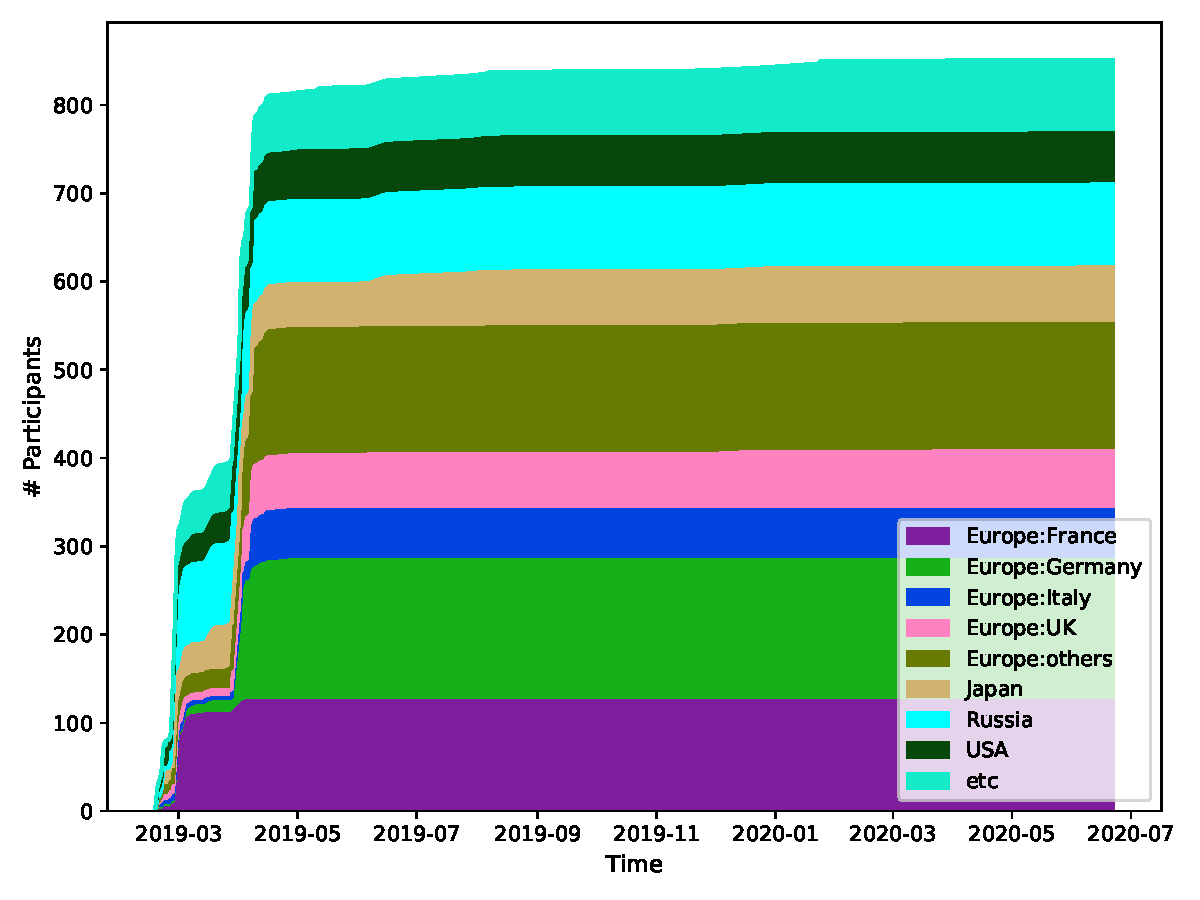
\includegraphics[width=12cm]{../pdfs/TimeSeries.pdf}
\caption{Time series}
\label{fig:timeseries}
\end{center}
\end{figure}
